\documentclass[11pt,twocolumn]{article}

\usepackage[hmargin=1.25cm, vmargin=1.5cm]{geometry} % Document margins

\usepackage{amsmath}
\usepackage{amsthm}
\usepackage{graphicx}
\usepackage{mathtools}
\usepackage{fullpage}
\usepackage{verbatim}

\title{Brownian Dynein Model}

\begin{document}

\maketitle

\section{Both bound}

\begin{figure}
  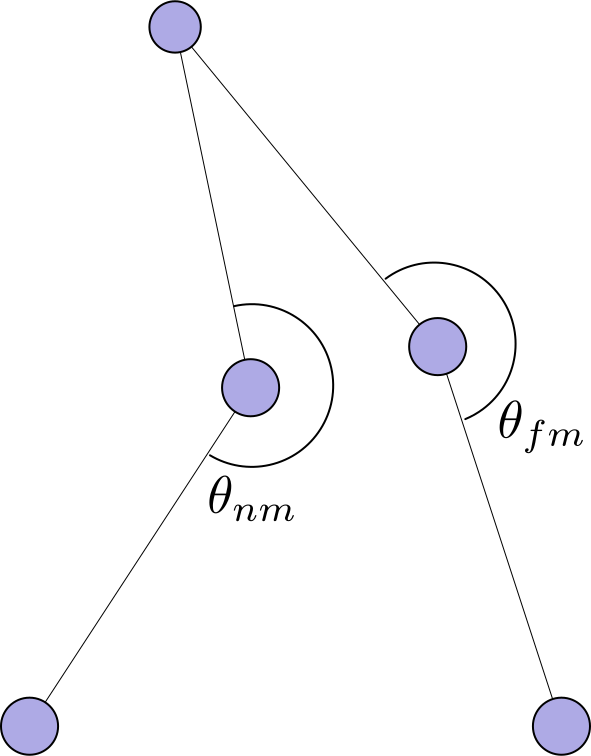
\includegraphics[width=\columnwidth]{../figures/code-bothbound}
  \caption{Angles used in both-bound case.}\label{fig:bothbound}
\end{figure}

In the both-bound case, we use two angles, as illustrated in
Fig.~\ref{fig:bothbound}.

These are the distances to the tail domain from the near and far
binding domains:
\begin{align}
  L_n &= \sqrt{L_s^2 + L_t^2 - 2L_sL_t\cos{\theta_{nm}}} \\
  L_f &= \sqrt{L_s^2 + L_t^2 - 2L_sL_t\cos{\theta_{fm}}}
\end{align}

\subsection{Nearbound and Tail coordinates}

We use two angles to determine the position of the motor domain:
\begin{align}
  \cos\theta_n &= \frac{L^2 + L_n^2 - L_f^2}{2L L_n} \\
  \sin\theta_{n} &= \sqrt{1 - \cos^2\theta_{n}} \\
  \cos\theta_{ns} &= \frac{L_s^2 + L_n^2 - L_t^2}{2L_s L_n} \\
  \sin\theta_{ns} &=
  \begin{cases}
    +\sqrt{1 - \cos^2\theta_{ns}} & \theta_{nm} < \pi \\
    -\sqrt{1 - \cos^2\theta_{ns}} & \theta_{nm} > \pi
  \end{cases}
\end{align}

and the derivatives are given by:

\begin{align}
  \frac{\partial \cos\theta_n}{\partial L_n} &= \frac{1}{L} - \frac{L^2 + L_n^2 - L_f^2}{2L L_n^2}\\
  \frac{\partial \cos\theta_n}{\partial L_f} &= -\frac{L_f}{LL_n}\\
  \frac{\partial \sin\theta_n}{\partial L_n} &= \frac{-\cos\theta_n}{\sqrt{1-\cos^2\theta_n}}
  \left(\frac{1}{L} - \frac{L^2 + L_n^2 - L_f^2}{2L L_n^2}\right)\\
  \frac{\partial \sin\theta_n}{\partial L_f} &= \frac{-\cos\theta_n}{\sqrt{1-\cos^2\theta_n}}
  \left(\frac{-L_f}{LLn}\right)\\
  \frac{\partial \cos\theta_{ns}}{\partial L_n} &= \frac{1}{L_s}
  - \frac{L_s^2 + L_n^2 - L_t^2}{2L_sL_n^2}\\
  \frac{\partial \cos\theta_{ns}}{\partial L_f} &= 0\\
  \frac{\partial \sin\theta_{ns}}{\partial L_n} &=
  \begin{cases}
    \frac{-\cos\theta_{ns}}{\sqrt{1-\cos^2\theta_{ns}}}
    \left(\frac{1}{L_s} - \frac{L_s^2+L_n^2-L_t^2}{2LL_n^2}\right) & \theta_{nm} < \pi \\
    \frac{\cos\theta_{ns}}{\sqrt{1-\cos^2\theta_{ns}}}
    \left(\frac{1}{L_s} - \frac{L_s^2+L_n^2-L_t^2}{2LL_n^2}\right) & \theta_{nm} > \pi
  \end{cases}\\
  \frac{\partial \sin\theta_{ns}}{\partial L_f} &= 0
\end{align}

Given these definitions, the position of the motor domain is given
simply by $\cos$ and $\sin$ of $\theta_n$ and $\theta_{ns}$:
\begin{align}
  X_{nm} &= L_s\left(
  \cos\theta_n\cos\theta_{ns} - \sin\theta_n\sin\theta_{ns}
  \right)
  \\
  Y_{nm} &= L_s\left(
  \cos\theta_n\sin\theta_{ns} + \sin\theta_n\cos\theta_{ns}
  \right)
  \\
  X_{t} &= L_n\cos\theta_n\\
  Y_{t} &= L_n\sin\theta_n\\
\end{align}

Looking at their derivatives gives:

\begin{multline}
  \frac{dX_{nm}}{dL_n} = L_s\Big(
  \cos\theta_n\frac{d\cos\theta_{ns}}{dL_n}
  + \cos\theta_{ns}\frac{d\cos\theta_{n}}{dL_n} \\
  - \sin\theta_n\frac{d\sin\theta_{ns}}{dL_n}
  - \sin\theta_{ns}\frac{d\sin\theta_{n}}{dL_n}
  \Big)\\
\end{multline}

\begin{multline}
  \frac{dY_{nm}}{dL_n} = L_s\Big(
  \cos\theta_n\frac{d\sin\theta_{ns}}{dL_n}
  + \sin\theta_{ns}\frac{d\cos\theta_{n}}{dL_n} \\
  + \sin\theta_n\frac{d\cos\theta_{ns}}{dL_n}
  + \cos\theta_{ns}\frac{d\sin\theta_{n}}{dL_n}
  \Big)
\end{multline}

\begin{multline}
  \frac{dX_{nm}}{dL_f} = L_s\Big(
  \cos\theta_n\frac{d\cos\theta_{ns}}{dL_f}
  + \cos\theta_{ns}\frac{d\cos\theta_{n}}{dL_f} \\
  - \sin\theta_n\frac{d\sin\theta_{ns}}{dL_f}
  - \sin\theta_{ns}\frac{d\sin\theta_{n}}{dL_f}
  \Big)
\end{multline}

\begin{multline}
  \frac{dY_{nm}}{dL_f} = L_s\Big(
  \cos\theta_n\frac{d\sin\theta_{ns}}{dL_f}
  + \sin\theta_{ns}\frac{d\cos\theta_{n}}{dL_f} \\
  + \sin\theta_n\frac{d\cos\theta_{ns}}{dL_f}
  + \cos\theta_{ns}\frac{d\sin\theta_{n}}{dL_f}
  \Big)
\end{multline}

\begin{align}
  \frac{dX_{t}}{dL_n} &= \cos\theta_n + L_n\frac{\partial \cos\theta_n}{\partial L_n} &= \frac{L_n}{L}\\
  \frac{dY_{t}}{dL_n} &= \sin\theta_n + L_n\frac{\partial \sin\theta_n}{\partial L_n}\\
  \frac{dX_{t}}{dL_f} &= L_n\frac{\partial \cos\theta_n}{\partial L_f} &= -\frac{L_f}{L}\\
  \frac{dY_{t}}{dL_f} &= L_n\frac{\partial \sin\theta_n}{\partial L_f}\\
\end{align}

The corresponding C++ code could look like:
\begin{verbatim}
  dXnm_dLn = Ls*(cosAn*dcosAns_dLn
                 + cosAns*dcosAn_dLn
                 - sinAn*dsinAns_dLn
                 - sinAns*dsinAn_dLn);
\end{verbatim}
Basically, we have lots of chain rules.\\

We then create a system of equations by equating velocities from Brownian dynamics to the velocities
we derived above:

\onecolumn

\begin{align}
  \dot{X}_{nm} &= \frac{1}{\gamma} \Big(F_{xml} - \lambda_{ns}(X_{bm} - X_{bb})
  + \lambda_{nt}(X_{t } - X_{bm}) \Big) + R_{xml}
  &=& \frac{\partial X_{nm}}{\partial L_n}\dot{L}_n + \frac{\partial X_{nm}}{\partial L_f}\dot{L}_f\\
  \dot{X}_{t } &= \frac{1}{\gamma} \Big(F_{xt } - \lambda_{nt}(X_{t } - X_{bm})
  + \lambda_{ft}(X_{fm} - X_{t }) \Big) + R_{xt }
  &=& \frac{\partial X_{t}}{\partial L_n}\dot{L}_n + \frac{\partial X_{t}}{\partial L_f}\dot{L}_f\\
  \dot{X}_{fm} &= \frac{1}{\gamma} \Big(F_{xmr} - \lambda_{ft}(X_{fm} - X_{t })
  + \lambda_{fs}(X_{fb} - X_{fm}) \Big) + R_{xmr}
  &=& \frac{\partial X_{fm}}{\partial L_n}\dot{L}_n + \frac{\partial X_{fm}}{\partial L_f}\dot{L}_f
\end{align}

\begin{align}
  \dot{Y}_{nm} &= \hspace{1cm} \frac{1}{\gamma} \Big(F_{yml} - \lambda_{ns}(Y_{bm} - Y_{bb})
  + \lambda_{nt}(Y_{t } - Y_{bm}) \Big) + R_{yml}
  &= \frac{\partial Y_{nm}}{\partial L_n}\dot{L}_n + \frac{\partial Y_{nm}}{\partial L_f}\dot{L}_f\\
  \dot{Y}_{t}  &= \hspace{1cm} \frac{1}{\gamma} \Big(F_{yt } - \lambda_{nt}(Y_{t } - Y_{bm})
  + \lambda_{ft}(Y_{fm} - Y_{t }) \Big) + R_{yt }
  &= \frac{\partial Y_{t}}{\partial L_n}\dot{L}_n + \frac{\partial Y_{t}}{\partial L_f}\dot{L}_f\\
  \dot{Y}_{fm} &= \hspace{1cm} \frac{1}{\gamma} \Big(F_{ymr} - \lambda_{ft}(Y_{fm} - Y_{t })
  + \lambda_{fs}(Y_{fb} - Y_{fm}) \Big) + R_{ymr}
  &= \frac{\partial Y_{fm}}{\partial L_n}\dot{L}_n + \frac{\partial Y_{fm}}{\partial L_f}\dot{L}_f
\end{align}

\twocolumn

\begin{figure}
  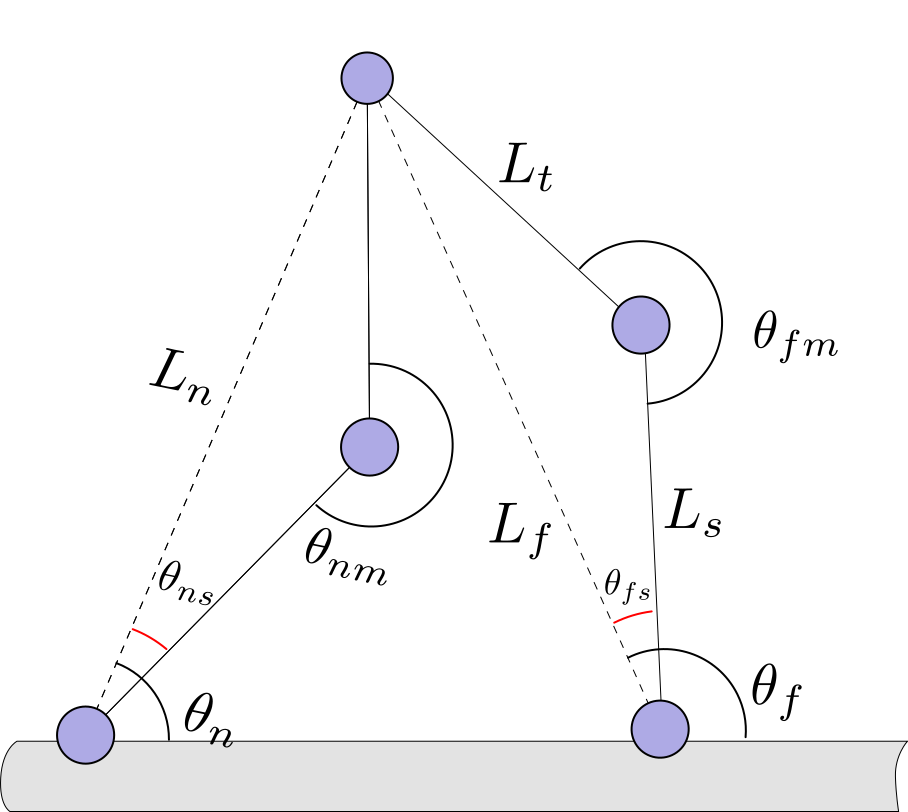
\includegraphics[width=\columnwidth]{../figures/similar-bothbound}
  \caption{Angles used in both-bound case.}\label{fig:similar}
\end{figure}

\subsection{Farbound coordinates}
The farbound coordinates are defined similarly (but not quite) to the nearbound coordinates, with
$L_n$ and $L_f$ coordinates switched places.
\begin{align}
  \cos\theta_f &= -\frac{L^2 + L_f^2 - L_n^2}{2L L_f}\\
  &\Bigg( \mbox{Or equivalently...   }
  \cos\left(\pi - \theta_f\right) &= \frac{L^2 + L_f^2 - L_n^2}{2L L_f}\Bigg)\\
  \sin\theta_{f} &= \sqrt{1 - \cos^2\theta_{f}} \\
  \cos\theta_{fs} &= \frac{L_s^2 + L_f^2 - L_t^2}{2L_s L_f} \\
  \sin\theta_{fs} &=
  \begin{cases}
    +\sqrt{1 - \cos^2\theta_{fs}} & \theta_{fm} < \pi \\
    -\sqrt{1 - \cos^2\theta_{fs}} & \theta_{fm} > \pi
  \end{cases}
\end{align}

The only change between the near and far coordinates (other than switching $L_n$ and $L_f$) is the
sign of $\cos\theta_{n/f}$. This is because, for positive L, $\theta_n$ is an internal angle and
$\theta_f$ is an external angle to the $L-L_n-L_f$ triangle. To properly deal with the $\theta_f$
angle, we must use its complement: $\pi - \theta_f$. The sign switch is because
$\cos\left(\pi - \theta_f\right) = -\cos\theta_f$.\\

For negative L values, the only change to the model is that $\theta_n$ becomes an external angle and
$\theta_f$ becomes internal. As we know, we must introduce a sign shift to account for this.
However we do not need to do any extra work, since the L in the denominator of $\cos\theta_f$
provides the necessary sign shift for $\theta_n$ going from internal to external.

\onecolumn

\section{Matrix Form}
Here we convert the above system into matrix form, solve it in Mathematica and list the results.

\[
\begin{pmatrix}
  -\frac{X_{nm}}{Ln} & -\frac{X_{nm}}{Lf}
  & -\frac{X_{nm}-X_{nb}}{\gamma} & \frac{X_{t}-X_{nm}}{\gamma} & 0 & 0\\
  -\frac{X_{t}}{Ln} & -\frac{X_{t}}{Lf}
  & 0 & -\frac{X_{t}-X_{nm}}{\gamma} & \frac{X_{fm}-X_{t}}{\gamma} & 0\\
  -\frac{X_{fm}}{Ln} & -\frac{X_{fm}}{Lf}
  & 0 & 0 & -\frac{X_{fm}-X_{t}}{\gamma} & \frac{X_{fb}-X_{fm}}{\gamma}\\
  -\frac{Y_{nm}}{Ln} & -\frac{Y_{nm}}{Lf}
  & -\frac{Y_{nm}-Y_{nb}}{\gamma} & \frac{Y_{t}-Y_{nm}}{\gamma} & 0 & 0\\
  -\frac{Y_{t}}{Ln} & -\frac{Y_{t}}{Lf}
  & 0 & -\frac{Y_{t}-Y_{nm}}{\gamma} & \frac{Y_{fm}-Y_{t}}{\gamma} & 0\\
  -\frac{Y_{fm}}{Ln} & -\frac{Y_{fm}}{Lf}
  & 0 & 0 & -\frac{Y_{fm}-Y_{t}}{\gamma} & \frac{Y_{fb}-Y_{fm}}{\gamma}\\
\end{pmatrix}
\begin{pmatrix}
  \dot{L}_n\\
  \dot{L}_f\\
  \lambda_{ns}\\
  \lambda_{nt}\\
  \lambda_{ft}\\
  \lambda_{fs}\\
\end{pmatrix}
=
\begin{pmatrix}
  -\frac{1}{\gamma}F_{nmx} - R_{nmx}\\
  -\frac{1}{\gamma}F_{tx}  - R_{tx}\\
  -\frac{1}{\gamma}F_{fmx} - R_{fmx}\\
  -\frac{1}{\gamma}F_{nmy} - R_{nmy}\\
  -\frac{1}{\gamma}F_{ty}  - R_{ty}\\
  -\frac{1}{\gamma}F_{fmy} - R_{fmy}\\
\end{pmatrix}
\]

\twocolumn

\section{Onebound}

\begin{figure}
  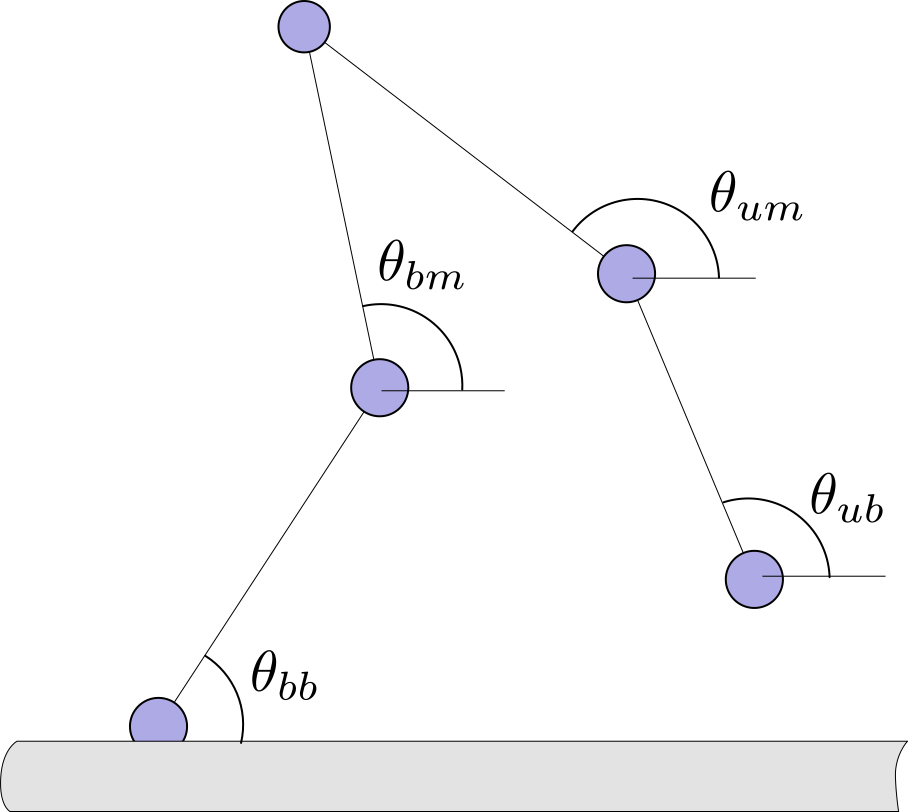
\includegraphics[width=\columnwidth]{../figures/code-onebound}
  \caption{Angles used in one-bound case.}\label{fig:onebound}
\end{figure}

First, some definitions...
\begin{align*}
F_{bmx} &= \frac{f_{bmx} + R_{bmx}}{\gamma}\\
F_{xt } &= \frac{f_{xt} + R_{xt}}{\gamma}\\
...\\
X_{bs} &= \frac{X_{bm} - X_{bb}}{\gamma}\\
X_{bt} &= \frac{X_t - X_{bm}}{\gamma}\\
...\\
\end{align*}

\subsection{Brownian Dynamics equations}
\begin{align*}
  \dot{X}_{bm} &= F_{bmx} - \gm\lambda_{bs}X_{bs} + \gm\lambda_{bt}X_{bt}\\
  \dot{X}_{t}  &= F_{tx}  - \gt\lambda_{bt}X_{bt} + \gt\lambda_{ut}X_{ut}\\
  \dot{X}_{um} &= F_{umx} - \gm\lambda_{ut}X_{ut} + \gm\lambda_{us}X_{us}\\
  \dot{X}_{ub} &= F_{ubx} - \gb\lambda_{us}X_{us}
\end{align*}

\begin{align*}
  \dot{Y}_{bm} &= F_{bmx} - \gm\lambda_{bs}Y_{bs} + \gm\lambda_{bt}Y_{bt}\\
  \dot{Y}_{t}  &= F_{tx}  - \gt\lambda_{bt}Y_{bt} + \gt\lambda_{ut}Y_{ut}\\
  \dot{Y}_{um} &= F_{umx} - \gm\lambda_{ut}Y_{ut} + \gm\lambda_{us}Y_{us}\\
  \dot{Y}_{ub} &= F_{ubx} - \gb\lambda_{us}Y_{us}
\end{align*}

\subsection{Expanded velocities}

\begin{align*}
\dot{X}_{bm} &= -L_s\sin(\theta_{bb})\dot{\theta}_{bb}\\
\dot{X}_{t } &= -L_s\sin(\theta_{bb})\dot{\theta}_{bb} - L_t\sin(\theta_{bm})\dot{\theta}_{bm}\\
\dot{X}_{um} &= -L_s\sin(\theta_{bb})\dot{\theta}_{bb} - L_t\sin(\theta_{bm})\dot{\theta}_{bm} + L_t\sin(\theta_{um})\dot{\theta}_{um}\\
\dot{X}_{ub} &= -L_s\sin(\theta_{bb})\dot{\theta}_{bb} - L_t\sin(\theta_{bm})\dot{\theta}_{bm} + L_t\sin(\theta_{um})\dot{\theta}_{um} + L_s\sin(\theta_{ub})\dot{\theta}_{ub}\\
\end{align*}

\begin{align*}
\dot{Y}_{bm} &= L_s\cos(\theta_{bb})\dot{\theta}_{bm}\\
\dot{Y}_{t } &= L_s\cos(\theta_{bb})\dot{\theta}_{bb} + L_t\cos(\theta_{bm})\dot{\theta}_{bm}\\
\dot{Y}_{um} &= L_s\cos(\theta_{bb})\dot{\theta}_{bb} + L_t\cos(\theta_{bm})\dot{\theta}_{bm} - L_t\cos(\theta_{um})\dot{\theta}_{um}\\
\dot{Y}_{ub} &= L_s\cos(\theta_{bb})\dot{\theta}_{bb} + L_t\cos(\theta_{bm})\dot{\theta}_{bm} - L_t\cos(\theta_{um})\dot{\theta}_{um} - L_s\cos(\theta_{ub})\dot{\theta}_{ub}\\
\end{align*}

\subsection{System of Equations}
Now to create our system of equations, we combine the Brownian equations with our expanded velocities. This system of equations takes into account both the dynamics of Brownian Mechanics (from the BD equations) as well as the constraints of our coordinate system (from the velocity expansions).

\begin{align*}
F_{bmx} - \gm\lambda_{bs}X_{bs} + \gm\lambda_{bt}X_{bt} &= -L_s\sin(\theta_{bb})\dot{\theta}_{bb}\\
F_{tx}  - \gt\lambda_{bt}X_{bt} + \gt\lambda_{ut}X_{ut} &= -L_s\sin(\theta_{bb})\dot{\theta}_{bb} - L_t\sin(\theta_{bm})\dot{\theta}_{bm}\\
F_{umx} - \gm\lambda_{ut}X_{ut} + \gm\lambda_{us}X_{us} &= -L_s\sin(\theta_{bb})\dot{\theta}_{bb} - L_t\sin(\theta_{bm})\dot{\theta}_{bm} + L_t\sin(\theta_{um})\dot{\theta}_{um}\\
F_{ubx} - \gb\lambda_{us}X_{us} &= -L_s\sin(\theta_{bb})\dot{\theta}_{bb} - L_t\sin(\theta_{bm})\dot{\theta}_{bm} + L_t\sin(\theta_{um})\dot{\theta}_{um} + L_s\sin(\theta_{ub})\dot{\theta}_{ub}\\
\\
F_{bmy} - \gm\lambda_{bs}Y_{bs} + \gm\lambda_{bt}Y_{bt} &= L_s\cos(\theta_{bb})\dot{\theta}_{bm}\\
F_{ty}  - \gt\lambda_{bt}Y_{bt} + \gt\lambda_{ut}Y_{ut} &= L_s\cos(\theta_{bb})\dot{\theta}_{bb} + L_t\cos(\theta_{bm})\dot{\theta}_{bm}\\
F_{umy} - \gm\lambda_{ut}Y_{ut} + \gm\lambda_{us}Y_{us} &= L_s\cos(\theta_{bb})\dot{\theta}_{bb} + L_t\cos(\theta_{bm})\dot{\theta}_{bm} - L_t\cos(\theta_{um})\dot{\theta}_{um}\\
F_{uby} - \gb\lambda_{us}Y_{us} &= L_s\cos(\theta_{bb})\dot{\theta}_{bb} + L_t\cos(\theta_{bm})\dot{\theta}_{bm} - L_t\cos(\theta_{um})\dot{\theta}_{um} - L_s\cos(\theta_{ub})\dot{\theta}_{ub}\\
\end{align*}


\subsection{Matrix form}

\[
\hspace{-2.5cm}
\begin{pmatrix}
  L_s\sin\theta_{bb} & 0 & 0 & 0 & -\gm X_{bs} & \gm\lambda_{bt}X_{bt} & 0 & 0\\
  L_s\sin(\theta_{bb}) & L_t\sin(\theta_{bm}) & 0 & 0 & 0 & -\gt X_{bt} & \gt X_{ut} & 0\\
  L_s\sin(\theta_{bb}) & L_t\sin(\theta_{bm}) & -L_t\sin(\theta_{um}) & 0 & 0 & 0 & -\gm X_{ut} & \gm X_{us}\\
  L_s\sin(\theta_{bb}) & L_t\sin(\theta_{bm}) & -L_t\sin(\theta_{um}) & -L_s\sin(\theta_{ub}) & 0 & 0 & 0 & -\gb X_{us}\\
  -L_s\cos(\theta_{bb}) & 0 & 0 & 0 & -\gm Y_{bs} & \gm Y_{bt} & 0 & 0\\
  -L_s\cos(\theta_{bb}) & -L_t\cos(\theta_{bm}) & 0 & 0 & 0 & -\gt Y_{bt} & \gt Y_{ut} & 0\\
  -L_s\cos(\theta_{bb}) & -L_t\cos(\theta_{bm}) & L_t\cos(\theta_{um}) & 0 & 0 & 0 & -\gm Y_{ut} & \gm Y_{us}\\
  -L_s\cos(\theta_{bb}) & -L_t\cos(\theta_{bm}) & L_t\cos(\theta_{um}) & L_s\cos(\theta_{ub}) & 0 & 0 & 0 & -\gb Y_{us}\\
\end{pmatrix}
\begin{pmatrix}
  \dot{\theta}_{bb}\\
  \dot{\theta}_{bm}\\
  \dot{\theta}_{um}\\
  \dot{\theta}_{ub}\\
  \lambda_{bs}\\
  \lambda_{bt}\\
  \lambda_{ut}\\
  \lambda_{us}\\
\end{pmatrix}
=
\begin{pmatrix}
  -F_{bmx}\\
  -F_{tx}\\
  -F_{umx}\\
  -F_{ubx}\\
  -F_{bmy}\\
  -F_{ty}\\
  -F_{umy}\\
  -F_{uby}\\
\end{pmatrix}
\]

\subsection{Mathematica input}
The above matrix equation can be represented as follows and solved via Mathematica:

\begin{align*}
AA &= L_s\sin\theta_{bb}      &  LL &= -L_s\cos(\theta_{bb})\\
BB &= L_t\sin(\theta_{bm})    &	 MM &= -L_t\cos(\theta_{bm})\\
CC &= -L_t\sin(\theta_{um})   &	 NN &= L_t\cos(\theta_{um})\\
DD &= -L_s\sin(\theta_{ub})   &	 OO &= L_s\cos(\theta_{ub})\\
\\
EE &= -\gm X_{bs}       &    PP &= -\gm Y_{bs}\\
FF &= \gm X_{bt}	    &	 QQ &= \gm Y_{bt}\\ 
GG &= -\gt X_{bt}	    &	 RR &= -\gt Y_{bt}\\
HH &= \gt X_{ut}	    &	 SS &= \gt Y_{ut}\\ 
II &= -\gm X_{ut}	    &	 TT &= -\gm Y_{ut}\\
JJ &= \gm X_{us}	    &	 UU &= \gm Y_{us}\\ 
KK &= -\gb X_{us}       &	 VV &= -\gb Y_{us}\\
\end{align*}

\[
\begin{pmatrix}
  AA & 0 & 0 & 0 & EE & FF & 0 & 0\\
  AA & BB & 0 & 0 & 0 & GG & HH & 0\\
  AA & BB & CC & 0 & 0 & 0 & II & JJ\\
  AA & BB & CC & DD & 0 & 0 & 0 & KK\\
  LL & 0 & 0 & 0 & PP & QQ & 0 & 0\\
  LL & MM & 0 & 0 & 0 & RR & SS & 0\\
  LL & MM & NN & 0 & 0 & 0 & TT & UU\\
  LL & MM & NN & OO & 0 & 0 & 0 & VV\\
\end{pmatrix}
V
=
\begin{pmatrix}
  X1\\
  X2\\
  X3\\
  X4\\
  X5\\
  X6\\
  X7\\
  X8\\
\end{pmatrix}
\]



\end{document}
